\documentclass[12pt]{scrartcl}
\usepackage{amsmath, amssymb, amsthm, mathtools}
\usepackage{enumitem}

\usepackage{tikz, pgfplots}
\pgfplotsset{compat=1.17, width=10cm}
\usepgfplotslibrary{external}
\tikzexternalize

\usepackage[OT1]{fontenc}
\usepackage{mlmodern}
\usepackage{setspace}

\usepackage[backend=biber,style=numeric,sortcites=true]{biblatex}
\addbibresource{main.bib}
\usepackage{hyperref}

\title{The Bigger The Better II}
\author{Group 8-29 \thanks{Derrick Lukimin (L, 2i204), Tan Yong Yih (2i222), Wu Hao (2i324), Darren Yap (2i425)}}
\date{2022}

\begin{document}
\onehalfspacing
\maketitle
\tableofcontents

\section{Introduction}
This project aims to find an algorithm to determine
the side length of the largest square that can be
inscribed inside a convex $n$-gon. It is a continuation from
a previous project completed in 2021, The Bigger The Better. \cite{tbtb1}

\subsection{Definitions}
\begin{description}[font=\bfseries, leftmargin=1cm, style=nextline]
\item[placement] A valid location, size and rotation of the square such that
all vertices of the square lie on the edges of the polygon.
\item[inscribed] All vertices of the square must lie on the edges of the polygon.
\item[RQ] Research Question
\end{description}

\subsection{Research Questions}
\begin{enumerate}
	\item What is the side length of the largest square that can be inscribed in a triangle?
	\item What is the side length of the largest square that can be inscribed in a regular $n$-gon, given $n \neq 4$?
	\item What is the side length of the largest square that can be inscribed in a convex $n$-gon?
\end{enumerate}

\subsection{Project Scope}
This project will only focus on convex polygons.

\section{Literature Review}
% stuff...

\clearpage

\section{Research Question 1}

RQ1 aims to find out the side length of the largest
square that can be inscribed in a triangle, given the side lengths of the triangle, $a$, $b$ and $c$. \\

Some key insights were found, which are: 
\begin{enumerate}
	\item It can be seen that no more than two vertices of a square can lie on a single side,
	      as a square has at most two co-linear vertices.
	\item We notice how a triangle has three sides, and a square has four vertices.
	      In order for all the vertices to lie on the triangle, using the Pigeonhole Principle,
	      there will be at least one side with two vertices lying on it.
	\item Combining the above insights, there will be one vertex of the square
	      each lying on two sides of the triangle, with the other two vertices of the square
	      lying on the latter side of the triangle.
\end{enumerate}

\clearpage

\subsection{Solution}
A figure has been constructed for the purposes of illustrating the following proof.
\begin{figure}[h!]
	\centering
	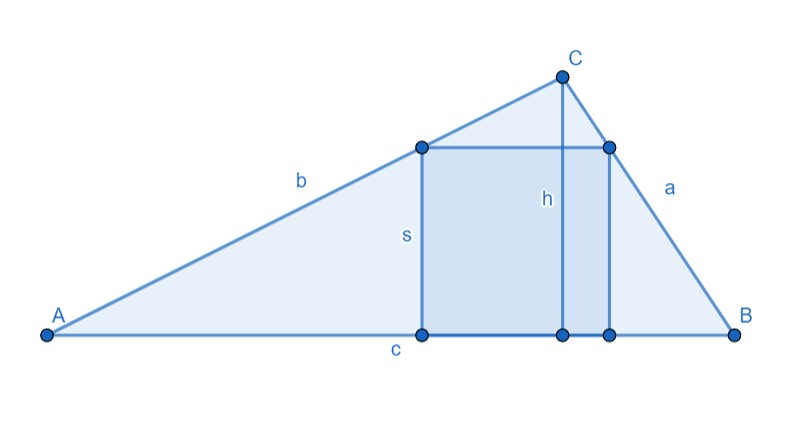
\includegraphics[scale=.75]{images/rq1.jpg}
	\label{fig:rq1_img}
	\caption{The figure for RQ1.}
\end{figure}

We see that side $c$ can be formed with $s$ as well as $s \cot A$ and $s \cot \angle B$.
\begin{align*}
	c & = s+s\cot \angle A+s\cot \angle B                                                                            
\end{align*}
We would like to express s in terms of side lengths a, b and c, as well as other values directly derived from the side lengths. \\
\begin{align*}
	s & = \frac{c}{1+\cot \angle A+\cot \angle B}                                                                      \\
	  & = \frac{c \sin\angle A}{\sin\angle A+\cos\angle A+\cot\angle B\sin\angle A}                                    \\
	  & = \frac{c\sin\angle A\sin\angle B}{\sin\angle A\sin\angle B+\cos\angle A\sin\angle B+\sin\angle A\cos\angle B} \\
	  & = \frac{c\sin\angle A\sin\angle B}{\sin\angle A\sin\angle B+\sin\left(\angle A+\angle B\right)}                \\
	  & = \frac{c\sin\angle A\sin\angle B}{\sin\angle A\sin\angle B+\sin\left(180-\angle C\right)}                     \\
	  & = \frac{c\sin\angle A\sin\angle B}{\sin\angle A\sin\angle B+\sin \angle C}                                     \\
	  & = \frac{2Rc\sin\angle A\sin\angle B}{2R\sin\angle A\sin \angle B+2R\sin \angle C}                              \\
	  & = \frac{ac\sin\angle B}{a\sin\angle B+c}                                                                       \\
	  & = \frac{2Rac\sin\angle B}{2Ra\sin\angle B+2Rc}                                                                 \\
	  & = \frac{abc}{2Rc+ab}                                                                                         
\end{align*}
We used formulae and theorems such as the sine addition formula and the law of sines to manipulate the expressions. \\

Since each of the sides of the triangle, $a$, $b$ and $c$ can be the longest side,
we can take the maximum of the three combinations, hence
\begin{equation}
	s_{\text{max}} = \max\left(\dfrac{abc}{2Rc+ab},\dfrac{abc}{2Rb+ac},\dfrac{abc}{2Ra+bc}\right)
\end{equation}

For obtuse triangles, we notice that only one placement exists, when the square lies on the longest side. We have:
\begin{equation}
	s = \dfrac{abc}{2Rc+ab}
\end{equation}
where c is the longest side.

\clearpage

\section{Research Question 2}

RQ2 aims to find out the side length of the largest
square that can be inscribed in a convex $n$-gon, given $n$ and the side length, $k$. \\

We have noticed that this problem can be split into 3 separate cases:
\begin{enumerate}
	\item when n is divisible by 4, 
	\item when n is divisible by 2 but not 4,
	\item when n is not divisible by 2.
\end{enumerate}
We shall tackle the cases in increasing order of difficulty.

\clearpage

\subsection{Case 1}

The first case is when n is divisible by 4. \\
This is the simplest case, as it can be seen that the diagonal of the square must be the same as the diagonal of the polygon. \\
Proof: The diagonal of the square connects 2 vertices of the square opposite to each other. It is the longest line segment in a square. 
Since the square has to be inscribed in the polygon, both ends of the diagonal have to lie on the edges of the polygon. 
It can be seen that the 2 furthest points on the edges of the polygon would be any vertex of the polygon and the opposite vertex. 
Hence, the diagonal of the square can be at most the length of the diagonal of the polygon. 
We can show that such a construction exists. \\

\begin{figure}[h!]
	\centering
	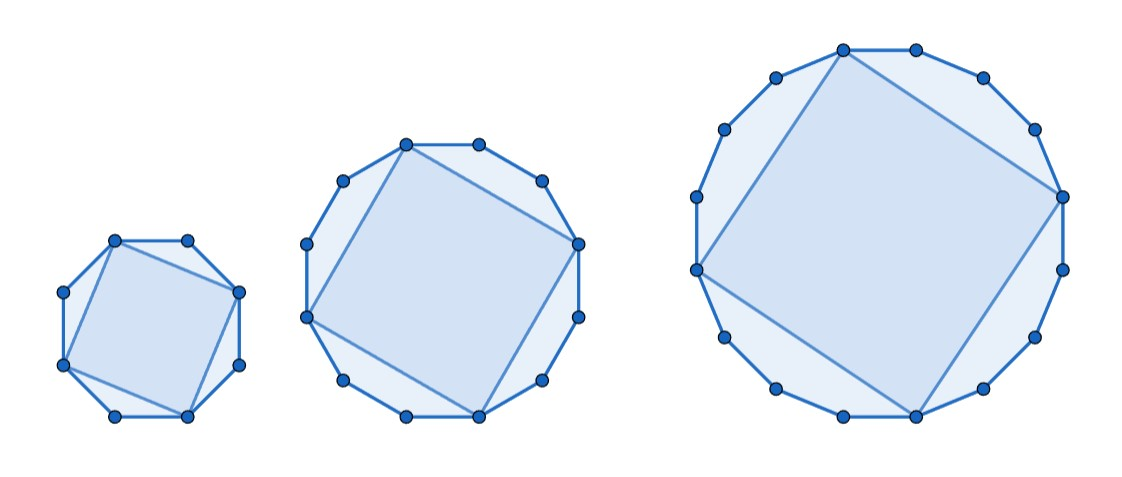
\includegraphics[scale=.75]{images/rq2_1_1.jpg}
	\label{fig:rq2_1_1_img}
	\caption{The constructions for case 1 of RQ2.}
\end{figure}

Hence, we can calculate the side length of the square. With reference to the figure, we shall calculate $l$ using the law of cosines. \\

\begin{figure}[h!]
	\centering
	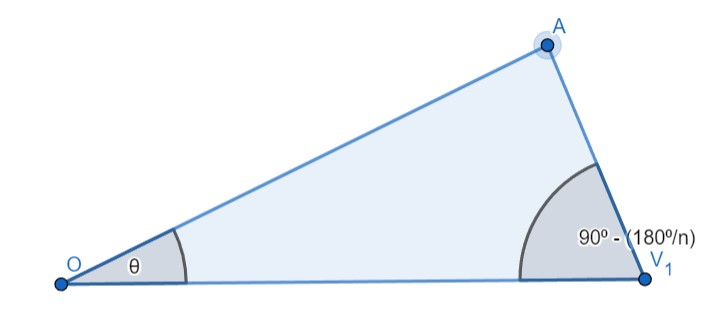
\includegraphics[scale=.75]{images/rq2_1_2.jpg}
	\label{fig:rq2_1_2_img}
	\caption{The figure for case 1 of RQ2.}
\end{figure}

\begin{align*}
	\angle AMB\ & =\ \frac{360^{\circ}}{2n}\      \\
	& =\ \frac{180^{\circ}}{n}          \\
	l^{2}+l^{2}-2\left(l\right)\left(l\right)\cos\left(\angle AMB\right) & =k^{2}    \\
	2l^{2}\left(1-\cos\left(\angle AMB\right)\right)\ & =k^{2}           \\
	l^{2} & =\frac{k^{2}}{2\left(1-\cos\left(\frac{180^{\circ}}{n}\right)\right)}   \\
	l\ & =\ k\sqrt{\frac{1}{2\left(1-\cos\left(\frac{180^{\circ}}{n}\right)\right)}}    \\
\end{align*}

Now, we can find $s$ using the Pythagoras theorem. \\

\begin{align*}
  2s^{2} & = \left(2l\right)^{2}    \\
	s^{2} & = 2l^{2}   \\
	s & = l\sqrt{2}    \\
	& = k\sqrt{\frac{2}{2\left(1-\cos\left(\frac{180^{\circ}}{n}\right)\right)}} \\
	& = k\sqrt{\frac{1}{\left(1-\cos\left(\frac{180^{\circ}}{n}\right)\right)}} \\
\end{align*}

\printbibliography
\end{document}
